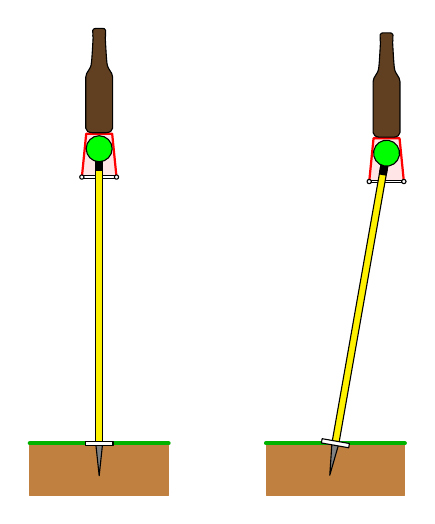
\begin{tikzpicture}[line cap=round,line join=round,>=stealth,x=1mm,y=1mm]

\def\ch{10} %cup height
\def\cdt{8} %cup top diameter
\def\cdb{6.0} %cup bottom diameter

\def\pl{70} %pole length actually 120
\def\pt{7.5} %pole taper length
\def\pd{1.6} %pole diameter
\def\dd{5} %disc diameter
\def\dt{1.9} %disc thickness
\def\balld{6.0} %tennis ball diameter
\def\extra{4} %how much to extend guide lines

\begin{scope}[scale=.55]

\draw (0,\pl-2) coordinate (B);

%ground
\draw[fill=brown,color=brown] (-4*\extra,-3*\extra) rectangle (4*\extra,0);
\draw[ultra thick, color=black!30!green] (-4*\extra,0) -- (4*\extra,0);

%cup
\draw (B) ++(0, \dt/2+2.5) coordinate(cup);
\draw[red,fill=red!10, thick] (cup) ++(-\cdt/2,-\ch) -- ++(\cdt/2-\cdb/2,\ch) -- ++(\cdb,0) -- ++(\cdt/2-\cdb/2,-\ch) -- cycle;
\draw[black,fill=white,thin] (cup) ++(-\cdt/2,-\ch-.3) rectangle ++(\cdt,.6);
\draw[black,fill=white,thin] (cup) ++(-\cdt/2,-\ch) circle (.5) ++(\cdt,0) circle (.5);

%pole
\draw[fill=yellow] (-\pd/2,0) rectangle ++(\pd,\pl); %pole
\draw[fill=black] (-\pd/2,\pl) rectangle ++(\pd,-\pl/10); %handle
\draw[fill=gray] (0,-\pt) -- ++(-\pd/2,\pt) -- ++(\pd,0) -- cycle; %spike
\draw[fill=white] (-2*\pd,-0.5) rectangle (2*\pd,0.5); %guard
\draw[fill=green] (B) circle (\balld/2); %tennis ball

%bottle
\begin{scope}[scale=.25]
\draw[fill=black!50!brown] 
(cup) ++(0,1)
 .. controls ++(-1,0) and ++(1,0) .. ++(-6.6,0)
.. controls ++(-3.2,0.2) and ++(0,-2.5) .. ++(-5.8, 4.2)
.. controls ++(0,1) and ++(0,-1) .. ++(0,47.2)
.. controls ++(0,2.5) and ++(-0.9,-1.4) .. ++(2.3,5.7)
.. controls ++(1.9,3.1) and ++(-0.3,-1.4)   .. ++(2.6,5.3)
 .. controls ++(0.5,2.1) and ++(-0.9,-16.8)  .. ++(1.9, 25.6) 
 .. controls ++(-0.4,0.4) and ++(-0.2,-1.1)  .. ++(-0.2, 3.3)
 .. controls ++(0.2,0.5) and ++(0.2,-0.2)  .. ++(-0.1,1.3) 
.. controls ++(-0.6,0.9) and ++(-1.1, -0.4)  .. ++(1.2,3.5) 
.. controls ++(1.2,0.4) and ++(-2.2,0)  .. ++(4.7, 0.2)

.. controls ++(2.2,0) and ++(-1.2,0.4) .. ++(4.7, -0.2)
 .. controls ++(1.1, -0.4) and ++(.6,0.9) .. ++(1.2,-3.5) 
 .. controls ++(-0.2,-0.2) and ++(-0.2,0.5) .. ++(-0.1,-1.3) 
 .. controls ++(0.2,-1.1) and ++(0.4,0.4) .. ++(-0.2, -3.3)
 .. controls ++(0.9,-16.8) and ++(-0.5,2.1) .. ++(1.9, -25.6) 
.. controls ++(0.3,-1.4) and ++(-1.9,3.1) .. ++(2.6,-5.3)
.. controls ++(0.9,-1.4) and ++(0,2.5) .. ++(2.3,-5.7) 
.. controls ++(0,-1) and ++(0,1) .. ++(0,-47.2)
.. controls ++(0,-2.5) and ++(3.2,0.2) .. ++(-5.8, -4.2) 
.. controls ++(-1,0) and ++(1,0) .. ++(-6.6,0)
;
\end{scope}
\end{scope}


\begin{scope}[xshift=30mm,scale=.55]

\draw[rotate=-10] (0,\pl-2) coordinate (B);

%ground
\draw[fill=brown,color=brown] (-4*\extra,-3*\extra) rectangle (4*\extra,0);
\draw[ultra thick, color=black!30!green] (-4*\extra,0) -- (4*\extra,0);

%cup
\draw (B) ++(0, \dt/2+2.5) coordinate(cup);
\draw[red,fill=red!10, thick] (cup) ++(-\cdt/2,-\ch) -- ++(\cdt/2-\cdb/2,\ch) -- ++(\cdb,0) -- ++(\cdt/2-\cdb/2,-\ch) -- cycle;
\draw[black,fill=white,thin] (cup) ++(-\cdt/2,-\ch-.3) rectangle ++(\cdt,.6);
\draw[black,fill=white,thin] (cup) ++(-\cdt/2,-\ch) circle (.5) ++(\cdt,0) circle (.5);

%pole
\begin{scope}[rotate=-10]
\draw[fill=yellow] (-\pd/2,0) rectangle ++(\pd,\pl); %pole
\draw[fill=black] (-\pd/2,\pl) rectangle ++(\pd,-\pl/10); %handle
\draw[fill=gray] (0,-\pt) -- ++(-\pd/2,\pt) -- ++(\pd,0) -- cycle; %spike
\draw[fill=white] (-2*\pd,-0.5) rectangle (2*\pd,0.5); %guard
\draw[fill=green] (B) circle (\balld/2); %tennis ball
\end{scope}

%bottle
\begin{scope}[scale=.25]
\draw[fill=black!50!brown] 
(cup) ++(0,1)
 .. controls ++(-1,0) and ++(1,0) .. ++(-6.6,0)
.. controls ++(-3.2,0.2) and ++(0,-2.5) .. ++(-5.8, 4.2)
.. controls ++(0,1) and ++(0,-1) .. ++(0,47.2)
.. controls ++(0,2.5) and ++(-0.9,-1.4) .. ++(2.3,5.7)
.. controls ++(1.9,3.1) and ++(-0.3,-1.4)   .. ++(2.6,5.3)
 .. controls ++(0.5,2.1) and ++(-0.9,-16.8)  .. ++(1.9, 25.6) 
 .. controls ++(-0.4,0.4) and ++(-0.2,-1.1)  .. ++(-0.2, 3.3)
 .. controls ++(0.2,0.5) and ++(0.2,-0.2)  .. ++(-0.1,1.3) 
.. controls ++(-0.6,0.9) and ++(-1.1, -0.4)  .. ++(1.2,3.5) 
.. controls ++(1.2,0.4) and ++(-2.2,0)  .. ++(4.7, 0.2)

.. controls ++(2.2,0) and ++(-1.2,0.4) .. ++(4.7, -0.2)
 .. controls ++(1.1, -0.4) and ++(.6,0.9) .. ++(1.2,-3.5) 
 .. controls ++(-0.2,-0.2) and ++(-0.2,0.5) .. ++(-0.1,-1.3) 
 .. controls ++(0.2,-1.1) and ++(0.4,0.4) .. ++(-0.2, -3.3)
 .. controls ++(0.9,-16.8) and ++(-0.5,2.1) .. ++(1.9, -25.6) 
.. controls ++(0.3,-1.4) and ++(-1.9,3.1) .. ++(2.6,-5.3)
.. controls ++(0.9,-1.4) and ++(0,2.5) .. ++(2.3,-5.7) 
.. controls ++(0,-1) and ++(0,1) .. ++(0,-47.2)
.. controls ++(0,-2.5) and ++(3.2,0.2) .. ++(-5.8, -4.2) 
.. controls ++(-1,0) and ++(1,0) .. ++(-6.6,0)
;
\end{scope}
\end{scope}
\end{tikzpicture}

